\documentclass[webpdf,modern,medium,namedate]{oup-authoring-template}

\usepackage[utf8]{inputenc}
\makeatletter
\setlength{\@fptop}{0pt}
\setlength{\@fpsep}{10pt plus 2pt minus 2pt}
\setlength{\@fpbot}{0pt plus 1fil}
\makeatother
\newcommand{\breakableurl}[1]{\url{#1}}
\graphicspath{{figures/}{paper/figures/}}

\journaltitle{Digital Scholarship in the Humanities}
\copyrightyear{2026}
\pubyear{2026}
\appnotes{Paper}
\firstpage{1}

\title[A Bilingual Latent Model of Proposition Hierarchy]{A Bilingual Latent Model of Proposition Hierarchy in Wittgenstein's Tractatus}

\author[1,$\ast$]{Mark A. Griffiths, MSc}
\authormark{Griffiths}
\address[1]{\orgdiv{Department of Academic Neuroscience}, \orgname{King's College London}, \orgaddress{\country{United Kingdom}}}
\corresp[$\ast$]{Corresponding author.}

\abstract{\textbf{Purpose:} This article asks whether the numbering of Wittgenstein's \emph{Tractatus} can provide weak structural supervision for text-conditioned latent representations of formal proposition position and bilingual correspondence within the retained German--English corpus. The aim is methodological: to make supplied formal organisation empirically inspectable, not to automate philosophical interpretation. \textbf{Design/methodology/approach:} Parent, depth, successor, and child-count targets are derived from proposition identifiers, while the encoder receives tokenised text only. The retained corpus contains 526 paired proposition IDs. A split-latent variational autoencoder is evaluated across ten seeds using random and lexical references, alignment-weight comparisons, wider-neighbourhood diagnostics, and rule-based, text-blind selection of family 2.2. \textbf{Findings:} Monolingual heads perform above retained-corpus references, and sibling propositions are closer than unrelated propositions. At $\lambda$ = 0.00, bilingual retrieval reaches Top-1 0.9348 and MRR 0.9650, above an exact-input character baseline. No or light alignment leaves formal-position distinctions largely intact, whereas high weights degrade retrieval and formal-position representation; shared parameters and surface cues prevent single-cause attribution. Wider neighbourhoods retain substantial overlap after the known counterpart is removed, and that selection identifies family 2.2 as cohesive but internally differentiated. All findings are retained-corpus diagnostics, not held-out tests. \textbf{Originality:} Within this shared architecture, hierarchy-derived supervision supports strong within-corpus bilingual proposition correspondence while preserving hierarchy-relevant distinctions in the low-pressure regime. \textbf{Contribution to the field of Digital Humanities:} The resulting representation does not interpret Wittgenstein's doctrines, but provides a reproducible framework for comparing proposition families, translation neighbourhoods, and candidate departures from formal structural expectations.}
\keywords{digital humanities; Tractatus Logico-Philosophicus; variational autoencoder; representation learning; textual hierarchy; bilingual alignment; computational philosophy; latent structure}

\begin{document}
\maketitle

\section*{Preprint status}
This manuscript is a preprint prepared for deposit in HAL and intended for submission to Digital Scholarship in the Humanities.

\section{Introduction}
The decimal architecture of Wittgenstein's Tractatus Logico-Philosophicus has long shaped attempts to reconstruct the organisation and progression of its philosophical argument. Although the relation between hierarchical and sequential readings remains contested, the proposition numbers identify explicit relations of depth, formal subordination, order, and textual neighbourhood that have informed debates about argumentative dependence and progression \citep{wittgenstein1922tractatus,hacker2015tractatus,kraft2016tractatus}. The numbering therefore matters not merely because it makes the work computationally convenient, but because textual form and questions of interpretive organisation are closely connected in the Tractatus. The present study treats this architecture as a formal research object rather than as a complete or uniquely correct philosophical interpretation.

The numbering already supplies parentage, depth, succession, and branch membership. The computational problem is therefore not to recover those labels from a lookup table, nor simply to classify proposition numbers. It is whether proposition text can be mapped into a compact, text-conditioned representation shaped by numbering-derived formal-position targets, so that recurring correspondences and departures between textual behaviour and formal organisation become inspectable across the corpus. Earlier computational work assembled multilingual versions of the Tractatus and visualised proposition-level similarity networks; the present study instead uses the numbering scaffold to supervise latent representation learning \citep{bucur2016tractatus}.

Here, \emph{weak structural supervision} means that labels are derived automatically from proposition identifiers rather than manually annotated from philosophical content, while the encoder receives only tokenised proposition text. The task is consequently supervised representation learning over a supplied formal scaffold. The model does not discover the hierarchy without labels, and the structure latent does not receive proposition IDs or hierarchy metadata as input; it is inferred from text under losses derived from that metadata.

The model is a split-latent variational autoencoder with recurrent encoder and decoder components \citep{kingma2014autoencoding,cho2014learning}. A 24-dimensional text latent supports reconstruction, while an 8-dimensional structure latent supports parent, depth, successor, and auxiliary child-count prediction. Parent and depth are hierarchy targets, child count describes direct subordinate structure, and the successor head represents ordered corpus position. In the fixed retained corpus the successor labels are nearly proposition-specific, so its accuracy is not directly comparable with the much coarser depth and parent tasks. The split encourages, but does not guarantee, a division of labour between surface reconstruction and formal-position prediction.

The monolingual experiment uses English proposition texts to ask how much numbering-derived information can be recovered from wording and how the resulting structure space organises formal relations. Its purpose is not to rank hierarchy and sequence by raw accuracy: the heads differ greatly in class number and imbalance. Rather, each head is interpreted relative to an appropriate retained-corpus reference level, while relational distances test whether local numbered families are represented differently from unrelated propositions.

The bilingual experiment holds numbered position constant while surface language changes. German and English texts are processed by a shared vocabulary, embedding table, encoder, decoder, and structural heads, and are trained against common formal-position target spaces. An optional pairwise loss directly attracts the posterior structure means of same-ID German and English samples when those samples co-occur within a minibatch. The $\lambda$ = 0 condition therefore removes direct same-ID attraction but remains a shared-parameter bilingual architecture. It tests whether explicit pairwise alignment is necessary in that setup; it does not isolate hierarchy supervision from shared parameters, reconstruction pressure, or lexical and symbolic overlap.

The learned representation adds something different from the numbering itself. A lookup table can recover the formal labels directly, whereas the model supplies text-conditioned latent neighbourhoods shaped by those labels. The present study demonstrates this use through a rule-based, text-blind proposition-family analysis and an aggregate comparison of German and English neighbourhoods after the known counterpart is removed. These analyses organise candidate cases and comparison sets for close reading, but proximity and neighbourhood overlap do not determine philosophical dependence or semantic equivalence.

The results show that all three categorical heads perform above their retained-corpus reference levels, while sibling propositions are substantially closer than unrelated propositions. The bilingual model achieves strong same-ID retrieval without an explicit pairwise loss and substantially exceeds an exact-input character n-gram reference, although that reference confirms non-trivial surface correspondence. After the known counterpart is excluded, the German and English versions retain substantial overlap in their wider proposition neighbourhoods. A small alignment weight consistently tightens matched posterior means but does not clearly improve retrieval or formal-position prediction, whereas heavier weighting damages correspondence, reconstruction, and relational organisation. Because the no-pairwise-loss condition still shares parameters, target spaces, and surface cues across languages, these results describe correspondence within a shared bilingual architecture rather than an effect of hierarchy supervision alone.

The principal contribution is methodological but interpretively enabling. Technically, the study uses a text-only encoder and proposition-number-derived formal-position targets to shape a compact structure-oriented latent. Empirically, it reports retained-corpus hierarchy, successor, geometry, bilingual retrieval, and wider-neighbourhood diagnostics, together with the effect of adding direct pairwise alignment. For scholarship, the rule-based, text-blind family analysis demonstrates how the latent artefacts can select regular and differentiated cases for subsequent examination. The method does not supply a philosophical interpretation of the Tractatus, establish language-invariant logic, or demonstrate generalisation beyond the retained texts.

The remainder of the paper situates the study within digital humanities work on Wittgenstein, explicit textual structure, structured humanities corpora, and representation learning. It then describes the corpus, information flow, split-latent architecture, alignment objective, training procedure, evaluation metrics, and exploratory case-selection procedure. The results report formal-position recovery, bilingual retrieval, wider-neighbourhood correspondence, reconstruction, latent-distance, child-count, PCA, and proposition-family diagnostics before the Discussion considers scholarly utility and limitations.

\section{Related Work}
\subsection{Digital humanities work on Wittgenstein and the Tractatus}
Digitisation has made Wittgenstein's writings available for computational analysis, scholarly editing, semantic modelling, and visualisation. The present study uses the German text and English translation of the \emph{Tractatus} supplied by Project Gutenberg \citep{projectgutenbergtractatus}. The wider manuscript corpus is available through the Wittgenstein Archives at the University of Bergen \citeyearpar{wittgenstein2016bergen}. Its interactive Nachlass edition presents linear clean-copy transcriptions alongside representations of insertions, deletions, overwriting, and other features of Wittgenstein's working documents. This broader context matters because computational analysis of Wittgenstein must remain attentive to textual organisation, manuscript transmission, editorial representation, and interpretive structure.

Two lines of research chiefly motivate the present study. First, \citet{bucur2016tractatus} assembled the German original and English, Spanish, French, and Russian translations of the \emph{Tractatus} and visualised proposition-level similarity networks within each language. The present study instead trains a text-conditioned neural representation using supervision derived from proposition numbering. The structure latent is not a direct encoding of proposition identifiers or hierarchy metadata: it is inferred from proposition text while being shaped by prediction targets derived from those identifiers.

Second, \citet{pichler2013sharing} used ontology methods to represent and retrieve relations in Wittgenstein's philosophy. Their symbolic approach encodes conceptual relations explicitly, whereas the present model learns latent geometry associated with formal textual position. The two methods therefore address different scholarly objects: explicit conceptual representation on the one hand, and text-conditioned formal organisation on the other.

\subsection{Explicit textual structure in digital humanities corpora}
Central to the current paper is that many key texts in humanities are not merely unstructured text, but also contain an inherent explicit textual architecture. This architecture may operate at various levels of abstraction and in the form of books, parts, chapters, sections, propositions, articles, objections, replies, scholia, notes, clauses, verses, lemmas, theorems, proofs, and commentary layers. Conventions in digital humanities, such as the Text Encoding Initiative (TEI), make this architecture tractable for online presentation and analysis through editorial markup, metadata and document schemas \citep{tei2026guidelines}.

In this paper, we treat the Tractatus proposition-numbering system as an especially clear example of explicit hierarchical structure in a text. Parent proposition, hierarchy depth, local proposition family, next proposition, and child count can all be derived from proposition number. Thus, this architecture allows for fine-grained control of structural supervision greater than that available for many other texts. However, the underlying principle is more general: structural information encoded through numbering, markup, or document schemas can provide analogous supervision in other formally organised corpora.

\subsection{Structured philosophical, legal, theological, and mathematical corpora}
The Tractatus is far from unique as a philosophical text with an explicit and distinct formal architecture. Spinoza’s Ethics is organised into parts, definitions, axioms, propositions, demonstrations, corollaries, scholia, and appendices \citep{spinoza1996ethics}. Aquinas’ Summa Theologiae is organised via questions, articles, objections, sed contra passages, respondeo sections, and replies \citep{aquinas1964summa}. These structures shape how argument, exposition, and response are distributed within each work. The split-latent VAE method used in the current study therefore permits us to ask whether various formal textual roles correspond to separable regions of latent space. Alternatively, we may ask whether analogous roles in different parts of a text exhibit similar representational patterns.

Legal, theological, mathematical, and technical corpora provide related cases of structured texts. Legal texts are often organised into acts, parts, chapters, articles, sections, clauses, recitals, and schedules, as in UK data-protection law \citeyearpar{uk2018dataprotection} and the GDPR \citeyearpar{eu2016gdpr}. Theological and canonical corpora may use stable reference systems such as book-chapter-verse in the Hebrew Bible, whose textual units can also be represented computationally through structured annotations and databases \citep{elliger1997bhs,roorda2017hebrew}. Mathematical texts distinguish definitions, lemmas, theorems, proofs, corollaries, examples, and remarks \citep{euclid1926elements,newton1999principia}. Technical standards and manuals often contain explicit procedural and hierarchical organisation. The method developed here is thus best understood as a general digital humanities approach to formally organised text, rather than as a model specific to Wittgenstein.

\subsection{Representation learning, weak supervision, and bilingual alignment}
The methodological contribution of the present study is to convert explicit document structure into automatically generated supervision targets for representation learning. Here, weak structural supervision refers to parent, depth, successor, and child-count labels derived deterministically from proposition identifiers rather than manually annotated from philosophical content. The encoder input remains proposition text only. The hierarchy is therefore not supplied as an input feature, but its derived labels shape the structure latent through supervised auxiliary objectives. This distinguishes the method from unsupervised topic modelling, lexical-similarity visualisation, and claims of metadata-free hierarchy discovery.

The bilingual German--English component extends this setup through a shared vocabulary, encoder, decoder, structural heads, and target spaces. German and English versions of the same proposition are distinct textual realisations of a known formal position. The experiment asks whether this shared architecture yields proposition-level correspondence and whether an additional pairwise loss changes that correspondence. The no-pairwise-loss condition is not an uncoupled language comparison, and the relative contributions of shared formal-position targets, shared parameters, reconstruction, and surface-form overlap cannot be separated without ablations. The task is consequently a constrained within-corpus test, not open-ended machine translation or a claim of multilingual philosophical reasoning.

\section{Method}
\subsection{Experimental Design}
The monolingual and bilingual experiments are two parts of the same supervised representation-learning study. The monolingual experiment asks whether an 8-dimensional structure latent inferred from English proposition text supports numbering-derived formal-position targets. The bilingual experiment asks whether German and English texts occupy a shared structure space within a common-parameter architecture, with and without an explicit same-ID pairwise loss. Neither experiment tests unsupervised discovery of philosophical meaning.

The principal evaluations are corpus-level diagnostics on the retained Tractatus proposition sets. No separate train/test split or held-out proposition-family split is used for the main claims. Stability is instead assessed by repeating retained configurations across random seeds and reporting seed-sweep means with SDs. All accuracy and retrieval results should therefore be read as retained-corpus representation rather than generalisation to unseen propositions.

\subsection{Corpus Construction and Numbering-Derived Targets}
The corpus was constructed from the Project Gutenberg electronic text of the Tractatus, which supplies the machine-readable source used for proposition extraction \citep{projectgutenbergtractatus}. The retained corpus contains 526 proposition IDs, with one English and one German text for every ID: 526 English rows, 526 German rows, and 1052 language-specific bilingual samples. The retained data contain no duplicate IDs or missing language counterparts.

The formal-position targets are deterministic functions of proposition identifiers and corpus order. Parent records the immediately superordinate proposition; depth records one of six observed hierarchical levels; the successor (next-proposition) target records the following proposition in reading order; and child count records the number of direct subordinate propositions. Children, siblings, and ancestor chains are also derived for relational diagnostics. German and English versions of the same proposition share these targets because they occupy the same numbered position.

The targets combine a tree-like hierarchy with ordered sequence. Parent has 169 observed target classes including the root grouping, depth has six observed classes, and the successor task has 526 observed labels across 526 propositions. The successor target is therefore close to a proposition-specific formal-position label in the retained corpus rather than a coarse measure of sequence. Raw accuracies across these heads are not interpreted as directly comparable measures of how strongly hierarchy and sequence are expressed.

A simplified bilingual row has this form:

\begin{center}
\begin{minipage}{0.96\columnwidth}
\footnotesize\ttfamily
\setlength{\parindent}{0pt}
id: "4.121"\\
parent\_id: "4.12"\\
depth: 4\\
texts.en: "Propositions cannot represent the\\
\hspace*{1.5em}logical form..."\\
texts.de: "Die Saetze koennen die logische\\
\hspace*{1.5em}Form nicht darstellen..."\\
next\_id: "4.1211"\\
children: ["4.1211", "4.1212"]\\
siblings: ["4.122", "4.123"]\\
ancestor\_chain: ["4", "4.1", "4.12"]\\
child\_count: 2
\end{minipage}
\end{center}

\subsection{Tokenisation and Text Representation}
Proposition text is lower-cased and tokenised at word level with punctuation retained as tokens. A vocabulary is built from the retained corpus, and tokens are mapped to integer IDs with padding, beginning-of-sequence, end-of-sequence, and unknown-token markers. The bilingual vocabulary contains 3913 entries including these special tokens, and German and English share the same learned token embedding table. The embeddings are corpus-specific rather than pretrained multilingual representations.

Encoded sequences are limited to 96 tokens including beginning- and end-of-sequence markers. In the retained bilingual corpus, 121 of 1052 language-specific samples exceed this limit and are truncated: 61 English and 60 German samples, representing 65 proposition IDs. Mini-batches are padded only to the longest retained sequence in each batch. Because the vocabulary is built with a minimum frequency of one from the retained texts, retained-corpus tokens are represented in the vocabulary; genuinely unseen tokens would map to the unknown marker.

\subsection{Split-Latent VAE Architecture}
The model is a recurrent variational autoencoder with gated recurrent unit encoder and decoder components \citep{cho2014learning}. The encoder receives only token IDs and sequence lengths; it does not receive proposition IDs, parent IDs, depth, successor labels, child count, sibling lists, or ancestor chains. Its final recurrent state is projected into separate means and log-variances for a 24-dimensional text latent and an 8-dimensional structure latent. Samples are drawn with the VAE reparameterisation trick \citep{kingma2014autoencoding}.

The decoder reconstructs proposition text from the text latent and does not receive the structure latent. In the bilingual model, a learned language embedding conditions whether German or English should be reconstructed. The intended division of labour is therefore that the text latent and language embedding support surface reconstruction, while the structure latent supports the formal-position heads. This architectural split encourages but does not guarantee complete disentanglement.

Parent, depth, and successor are categorical prediction tasks operating on the structure latent. Child count is an auxiliary scalar regression task trained with mean squared error. The labels are supplied as training targets only: the structure latent is text-conditioned and shaped by metadata-derived losses, rather than being a direct encoding of metadata. The shared heads constitute a multitask objective over related formal-position labels \citep{caruana1997multitask}.

\subsection{Bilingual Conditioning and Structure Alignment}
The bilingual model shares its vocabulary, token embeddings, encoder, decoder, structural heads, target label spaces, and optimisation schedule across German and English samples. Each sample also carries a language ID used only to condition reconstruction through the language embedding. Consequently, the $\lambda$ = 0 condition still couples the two languages through common parameters, common target spaces, mixed-corpus training, and shared lexical or symbolic features.

Where enabled, the explicit alignment objective operates on posterior means of the structure latent rather than stochastic samples. Within each shuffled minibatch, German and English samples sharing a proposition index are identified, and mean squared error is calculated between their posterior structure means. The term contributes only when matched samples co-occur; paired batching is not enforced. At $\lambda$ = 0, no same-ID pair is directly compared by this objective. The sweep over $\lambda$ = 0.00, 0.03, 0.10, 0.30, and 1.00 therefore tests the additional effect of direct pairwise attraction within an already shared bilingual architecture, not the isolated causal effect of hierarchy supervision.

\subsection{Training Objectives and Experimental Settings}
The retained monolingual setting uses a 24-dimensional text latent, an 8-dimensional structure latent, $\beta_{\mathrm{text}}$ = 0.01, and $\beta_{\mathrm{structure}}$ = 0.05. The bilingual objective combines reconstruction loss; separate KL penalties for the text and structure latents; parent, depth, successor, and child-count losses; and, where enabled, the pairwise alignment loss. The retained bilingual sweep uses $\beta_{\mathrm{text}}$ = 0.01, $\beta_{\mathrm{structure}}$ = 0.05, $\lambda_{\mathrm{parent}}$ = 0.2, $\lambda_{\mathrm{depth}}$ = 0.1, $\lambda_{\mathrm{next}}$ = 0.2, and $\lambda_{\mathrm{child}}$ = 0.02, while varying only the alignment weight.

Comparison across alignment strengths is descriptive rather than an automated model-selection procedure. No condition is treated as statistically decisive on the basis of a single metric. The no-pairwise-loss and $\lambda$ = 0.03 conditions are interpreted as practically comparable low-pressure settings on the principal retrieval and formal-position outcomes.

\subsection{Evaluation, Reference Levels, and Statistical Reporting}
Reconstruction is measured with token-level loss and perplexity. Parent, depth, and successor prediction are evaluated with accuracy. Because the three classification tasks differ sharply in granularity and class balance, their raw accuracies are contextualised with retained-corpus reference levels calculated over the observed target classes. Majority-class accuracy is 0.0266 for parent, 0.4658 for depth, and 0.0019 for successor; uniform accuracy over the observed classes is 0.0059, 0.1667, and 0.0019 respectively. Balanced accuracy and macro-F1 supplement overall accuracy for parent and depth, while Top-$k$, MRR, and rank diagnostics supplement Top-1 accuracy for the fine-grained parent and successor tasks. These are descriptive retained-corpus diagnostics, not held-out baselines.

Child count is evaluated with mean absolute error (MAE) and root mean squared error (RMSE). Since 68.1\% of propositions have zero direct children, performance is compared with constant mean and constant median (zero) predictors rather than a rounded count classification. The child-count diagnostics were computed from the retained seed-sweep checkpoints.

Cross-language evaluation uses deterministic posterior structure means. In German-to-English retrieval, a German mean is the query and all 526 English means are ranked by Euclidean distance; English-to-German retrieval reverses the direction. Top-1 records whether the nearest item has the same proposition ID, and mean reciprocal rank (MRR) records the reciprocal rank of that item. For 526 candidates, random Top-1 chance is 0.0019 and expected random MRR is 0.0130. Proposition IDs are used only after latent vectors have been produced, to score retrieval ranks.

Same-ID distance is the mean Euclidean distance between German and English posterior structure means for the same proposition. It is related to, but not numerically identical with, the mean-squared-error alignment objective used during training. Directional retrieval and by-language formal-position accuracies are reported separately to assess whether either language appears to be a privileged anchor.

For an exploratory comparison of the two low-pressure settings, differences between $\lambda$ = 0.03 and $\lambda$ = 0.00 were paired by seed and 95\% bootstrap confidence intervals were calculated with 10,000 resamples. These post hoc intervals characterise effect size and uncertainty rather than establish a formal model-selection result. Exact-input lexical retrieval baselines use the same text spans retained under the 96-token model limit, exclude proposition identifiers, and rank all 526 candidates in each direction. Exact-token Jaccard, word TF--IDF cosine, and character 3--5-gram TF--IDF cosine provide deterministic surface-form reference levels.

The structure latent is also analysed with relational distances and PCA. Parent-child distances are structural-role diagnostics rather than graph-geodesic distances required to be shorter than unrelated-pair distances. PCA projections are representative single-seed diagnostics, not aggregate evidence. Quantitative claims are based on ten-seed sweeps: seeds 0--9 for the monolingual model and for every bilingual alignment weight. Reported dispersions are sample standard deviations across seeds.

\subsection{Exploratory Proposition-Level Analysis}
To demonstrate how the retained representation can organise proposition-level scholarly investigation, a rule-based, text-blind analysis was conducted using cached posterior structure means. Immediate-parent families containing four to ten children were eligible. Pairwise sibling distances were calculated separately across ten monolingual seeds and compared with 5,000 randomly assembled proposition sets matched on child-depth profile and top-level branch. Candidate families and recurrent within-family differentiation were ranked from IDs, formal metadata, distances, text lengths, and truncation flags before proposition wording was joined to the analysis. The procedure is an exploratory retained-corpus demonstration rather than a held-out or preregistered test.

For the bilingual extension, neighbourhoods were compared at $k$ = 5, 10, and 20 under the $\lambda$ = 0.00 and 0.03 conditions. Same-language comparisons contrast the proposition IDs surrounding the German query in German space with those surrounding the English query in English space. Cross-direction comparisons contrast German-to-English and English-to-German neighbour-ID sets. The query itself and, for cross-language comparisons, the known same-ID counterpart were excluded. Jaccard overlap was aggregated across ten seeds and compared with independently permuted neighbour sets. These diagnostics ask whether corresponding language versions retain similar wider representational contexts; they do not treat overlap as semantic or philosophical equivalence.

\section{Results}
The following results are retained-corpus diagnostics from ten independently seeded runs, reported as means with sample standard deviations. Because the formal-position heads differ substantially in target granularity and class balance, their accuracies are interpreted against task-specific reference levels rather than treated as directly comparable measures of difficulty. The no-pairwise-loss result establishes that direct same-ID attraction is unnecessary within the shared bilingual architecture; it does not attribute correspondence to hierarchy supervision alone. These results concern constrained representation learning, not comprehension of Wittgenstein's logic.

\subsection{Monolingual Split-Latent Results}
Table 1 and Figure 1 report the monolingual seed sweep. Parent accuracy is 0.6983 $\pm$ 0.0152, compared with a retained-corpus majority reference of 0.0266. The correct parent appears among the five highest-scoring classes with accuracy 0.8848 $\pm$ 0.0113. Balanced accuracy (0.4204 $\pm$ 0.0193) and macro-F1 (0.3764 $\pm$ 0.0217) are lower than overall accuracy, indicating substantial but uneven recovery across the 169 observed parent classes.

Depth accuracy is 0.9274 $\pm$ 0.0275, compared with a majority reference of 0.4658. Balanced accuracy is 0.7107 $\pm$ 0.0690, mean absolute depth error is 0.1015 $\pm$ 0.0375, and approximately 68\% of incorrect predictions differ from the target by one level. The retained latent therefore carries a strong signal for broad depth, without establishing that a hierarchical philosophical reading is superior.

Successor prediction involves 526 observed, nearly proposition-specific targets. Top-1 accuracy is 0.3724 $\pm$ 0.0198, far above its 0.0019 random reference; the correct successor is within the top ten predictions in 0.8160 $\pm$ 0.0181 of cases, MRR is 0.5177 $\pm$ 0.0139, and mean rank is 8.11 $\pm$ 0.53. These rank diagnostics show considerable proposition-specific information even when the exact successor is not ranked first. Incorrect predictions are not generally confined to immediate reading-order neighbours: the mean of the per-seed median displacements is approximately 68 propositions, and only about 10.7\% remain within the correct parent family. The head is therefore evidence of successor-label discrimination, not a smooth latent geometry of reading order. Raw accuracy across depth, parent, and successor should not be treated as a commensurable ranking of hierarchy and sequence.

The relational diagnostics add information that class accuracy alone does not provide. Sibling propositions are closer than the deterministic unrelated comparison set in all ten seeds. The unrelated-minus-sibling contrast is 3.4919 $\pm$ 0.0460, providing robust retained-corpus evidence that local numbered families correspond to distinct latent organisation. Parent-child distance is instead 0.5491 $\pm$ 0.1560 greater than unrelated distance. The model is therefore not a literal graph embedding in which every direct tree edge must be short: its heads discriminate roles and labels without imposing graph-geodesic distance. This geometry provides a principled basis for asking which formal families are especially cohesive or contain outliers, but it does not establish philosophical dependence.

The auxiliary child-count head achieves MAE 0.5181 $\pm$ 0.0319 and RMSE 0.7602 $\pm$ 0.0468, substantially outperforming the constant predictors reported in Table 8. Performance is uneven across the zero-skewed target: MAE is 0.3163 $\pm$ 0.0238 for zero-child propositions and 0.9481 $\pm$ 0.0664 for propositions with one or more children. This is evidence of retained-corpus count information rather than uniform recovery across the full range of branching structures.

\begin{table}[htbp]
\centering
\caption{Monolingual seed-sweep summary for the retained split-latent configuration across seeds 0--9. Values are mean $\pm$ sample SD. Raw accuracies should be interpreted with the task granularity and reference levels in Table 2: depth has six observed classes, parent has 169, and successor has 526. Task-specific imbalance and rank diagnostics are reported in the text. Reconstruction and distance metrics are retained-corpus diagnostics. Parent-child distance is not expected to reproduce every direct tree edge as a short geometric relation.}

\begin{tabular}{lc}
\toprule
Metric & Value \\
\midrule
Seeds & 10 (0-9) \\
Parent accuracy & 0.6983 $\pm$ 0.0152 \\
Depth accuracy & 0.9274 $\pm$ 0.0275 \\
Successor accuracy & 0.3724 $\pm$ 0.0198 \\
Reconstruction loss & 1.2923 $\pm$ 0.0194 \\
Perplexity & 3.6416 $\pm$ 0.0706 \\
KL structure & 8.9653 $\pm$ 0.1127 \\
Sibling distance & 2.0656 $\pm$ 0.0342 \\
Parent-child distance & 6.1065 $\pm$ 0.1566 \\
Unrelated distance & 5.5574 $\pm$ 0.0532 \\
\botrule
\end{tabular}
\end{table}

\begin{figure}[htbp]
\centering
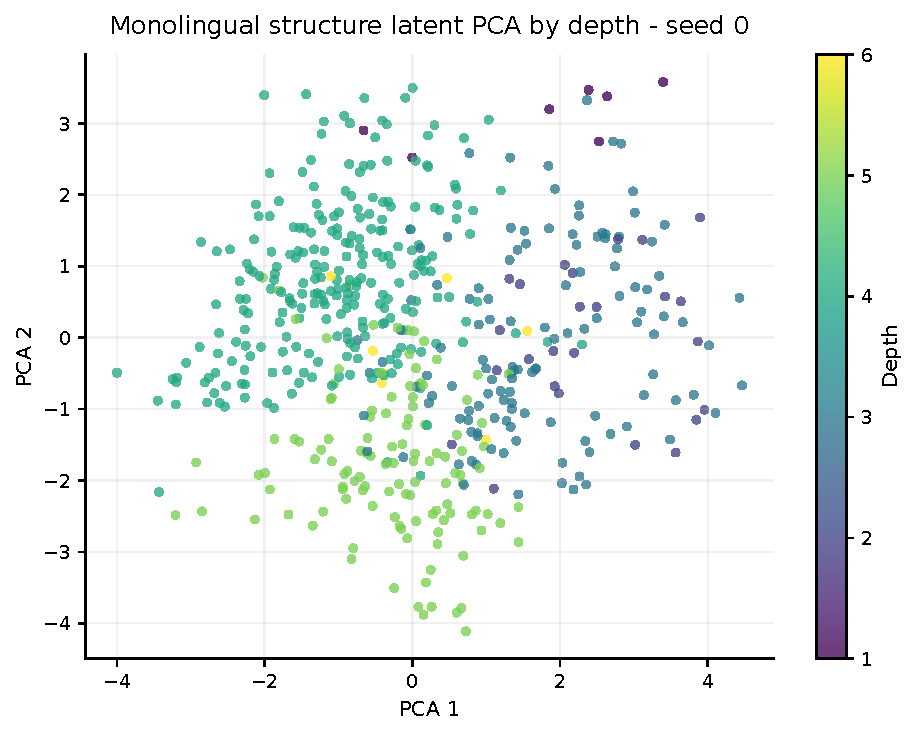
\includegraphics[width=0.84\linewidth]{monolingual_latent_pca_depth_reg005_seed000.pdf}
\caption{PCA projection of the 8D monolingual structure latent for representative seed 0, coloured by proposition depth. This single-seed visual diagnostic should be read alongside the aggregate metrics and task reference levels in Tables 1 and 2.}
\end{figure}

\begin{table*}[t]
\centering
\caption{Retained-corpus reference levels for the categorical formal-position tasks. Observed classes report the targets present in the 526-proposition corpus. Majority and uniform accuracies are descriptive reference levels rather than held-out baselines. The monolingual and bilingual values reproduce the retained seed-sweep means for comparison.}
\begin{tabular}{lccccc}
\toprule
Task & Classes & Majority & Uniform & Mono. & Bilingual $\lambda$=0 \\
\midrule
Parent & 169 & 0.0266 & 0.0059 & 0.6983 & 0.8601 \\
Depth & 6 & 0.4658 & 0.1667 & 0.9274 & 0.9646 \\
Successor & 526 & 0.0019 & 0.0019 & 0.3724 & 0.6202 \\
\botrule
\end{tabular}
\end{table*}

\subsection{Bilingual Alignment Results}
The bilingual experiment asks whether a common-parameter German--English model supports same-ID correspondence while retaining formal-position information. The core seed-sweep results are reported in Table 3 and visualised in Figure 2. At $\lambda$ = 0.00, where no pairwise same-ID loss is active, Top-1 retrieval is 0.9348 $\pm$ 0.0115 and MRR is 0.9650 $\pm$ 0.0066, compared with random reference levels of 0.0019 and 0.0130. This condition still shares vocabulary, embeddings, encoder, decoder, structural heads, label spaces, and mixed-corpus training across languages. It therefore shows that direct pairwise attraction is unnecessary in this architecture, not that hierarchy supervision alone caused the correspondence.

Exact-input surface baselines provide a stronger reference than random ranking (Table 9). Character 3--5-gram TF--IDF reaches mean Top-1 accuracy 0.4097 and MRR 0.5239 across directions; exact-token Jaccard reaches 0.1768 and 0.2539, and word TF--IDF reaches 0.1293 and 0.1941. The $\lambda$ = 0.00 structure latent remains substantially higher at 0.9348 and 0.9650. Simple surface correspondence is therefore non-trivial but does not reproduce the learned latent retrieval. The remaining difference cannot be attributed exclusively to hierarchy supervision because shared parameters, reconstruction pressure, and the nearly proposition-specific successor targets are also present.

The wider-neighbourhood analysis extends evaluation beyond recovery of the known counterpart (Table 10). At $k$ = 10 and $\lambda$ = 0.00, the mean Jaccard overlap between German-to-English and English-to-German neighbour-ID sets was 0.6240 $\pm$ 0.0086 across seeds after the same-ID counterpart was excluded. The corresponding overlap between the German and English within-language neighbourhoods was 0.6301 $\pm$ 0.0062, compared with an expected Jaccard of approximately 0.0103 for independent random ten-item sets. At $\lambda$ = 0.03, cross-direction overlap was 0.6270 $\pm$ 0.0086 and within-language overlap 0.6303 $\pm$ 0.0055. Light pairwise alignment therefore made little difference to aggregate wider-neighbourhood correspondence. The shared representation preserves considerable proposition-level context beyond the known match, but the result does not establish translation equivalence or isolate the contributions of common targets, shared parameters, and surface cues.

At $\lambda$ = 0.03, retrieval means are numerically slightly higher: 0.9365 $\pm$ 0.0103 for Top-1 and 0.9662 $\pm$ 0.0058 for MRR. The paired mean differences are only 0.0017 for Top-1 (95\% bootstrap CI $-0.0014$ to 0.0048) and 0.0012 for MRR (95\% CI $-0.0004$ to 0.0029). The no-pairwise-loss and light-alignment conditions are therefore practically similar on the principal retrieval outcomes.

Light alignment nevertheless has a consistent local effect on matched pairs. Same-ID distance falls from 0.7598 $\pm$ 0.0195 at $\lambda$ = 0.00 to 0.7486 $\pm$ 0.0173 at $\lambda$ = 0.03, a paired reduction of 0.0112 (95\% bootstrap CI 0.0083 to 0.0138) observed in all ten seeds. Parent, depth, and successor accuracies change only marginally over the same comparison. The pairwise term therefore tightens same-ID posterior means at low weight without producing a clear gain in the principal retrieval or formal-position metrics.

Increasing the weight beyond $\lambda$ = 0.03 does not continue to tighten matched pairs. Same-ID distance rises to 0.7756 at $\lambda$ = 0.10, 0.9502 at $\lambda$ = 0.30, and 1.1970 at $\lambda$ = 1.00. Retrieval, reconstruction, and all formal-position heads deteriorate over the same range. At $\lambda$ = 1.00, Top-1 falls to 0.7943 $\pm$ 0.0188, MRR to 0.8577 $\pm$ 0.0130, parent accuracy to 0.5736 $\pm$ 0.0340, depth accuracy to 0.7984 $\pm$ 0.0415, and successor accuracy to 0.3614 $\pm$ 0.0213. Heavy weighting therefore disrupts both realised correspondence and formal-position representation rather than achieving progressively greater invariance. The retained outputs do not establish the optimisation mechanism responsible for this deterioration.

The auxiliary child-count results follow the same broad pattern (Table 8). The no-pairwise-loss and light-alignment conditions give nearly identical MAE and RMSE, whereas both errors increase under heavier alignment. The head remains well above the constant-predictor reference levels, but its deterioration supplies an additional retained-corpus indication that high pairwise weights weaken formal-position information.

German-to-English and English-to-German retrieval are closely matched in aggregate. Table 4 shows small directional differences in Top-1 and MRR, while Table 5 shows similarly close aggregate German--English formal-position accuracies. This is consistent with reciprocal organisation in the shared model rather than an obvious directionally privileged mapping, although aggregate balance does not exclude proposition-level asymmetries. It does not establish semantic equivalence between the German and English texts.

Reconstruction and latent diagnostics clarify the high-weight pattern. Table 6 and Figure 5 show broadly stable reconstruction under no or light pairwise pressure and deterioration at larger weights. Table 7 shows a non-uniform reorganisation of geometry: sibling distances increase while parent-child, cross-language parent-child, and unrelated distances decrease. Auxiliary audit diagnostics also show declining structure-mean norms and increasing posterior variance. The pattern is therefore better described as degraded relational organisation than uniform compression.

The PCA projection in Figure 6 provides a representative visual diagnostic for the $\lambda$ = 0.03, seed 0 condition coloured by language. German and English samples occupy the same broad projected regions, but this single-seed projection does not distinguish the effects of common targets, shared model parameters, and lexical or symbolic cues. The principal bilingual evidence is the ten-seed pattern across Tables 3--10.

Taken together, the bilingual results demonstrate strong retained-corpus same-ID correspondence without direct pairwise attraction in a shared-parameter model trained on common formal-position targets. Neural retrieval is far above both random ranking and the strongest exact-input surface baseline, but the experiment does not causally isolate hierarchy supervision from shared parameters, reconstruction pressure, the nearly proposition-specific successor objective, or surface-form overlap. Light pairwise alignment modestly tightens matched means; heavy weighting damages correspondence and relational organisation. None of these findings establishes semantic equivalence, general multilingual transfer, or philosophical understanding.

\begin{table*}[htbp]
\centering
\caption{Core bilingual seed-sweep metrics across language-alignment weights. $\lambda$ is the optional same-proposition German--English alignment weight. Parent, depth, and successor accuracy evaluate the formal-position heads; Top-1 and MRR evaluate cross-language same-ID retrieval. All metric values are mean $\pm$ SD across seeds 0--9.}

\resizebox{\textwidth}{!}{%
\begin{tabular}{lcccccc}
\toprule
Lambda & Seeds & Parent accuracy & Depth accuracy & Successor accuracy & Top-1 & MRR \\
\midrule
0.00 & 10 (0-9) & 0.8601$\pm$ 0.0094 & 0.9646$\pm$ 0.0133 & 0.6202$\pm$ 0.0194 & 0.9348$\pm$ 0.0115 & 0.9650$\pm$ 0.0066 \\
0.03 & 10 (0-9) & 0.8608$\pm$ 0.0094 & 0.9643$\pm$ 0.0136 & 0.6189$\pm$ 0.0219 & 0.9365$\pm$ 0.0103 & 0.9662$\pm$ 0.0058 \\
0.10 & 10 (0-9) & 0.8539$\pm$ 0.0102 & 0.9574$\pm$ 0.0166 & 0.6142$\pm$ 0.0237 & 0.9227$\pm$ 0.0087 & 0.9546$\pm$ 0.0043 \\
0.30 & 10 (0-9) & 0.8029$\pm$ 0.0110 & 0.9320$\pm$ 0.0249 & 0.5596$\pm$ 0.0190 & 0.8720$\pm$ 0.0112 & 0.9143$\pm$ 0.0080 \\
1.00 & 10 (0-9) & 0.5736$\pm$ 0.0340 & 0.7984$\pm$ 0.0415 & 0.3614$\pm$ 0.0213 & 0.7943$\pm$ 0.0188 & 0.8577$\pm$ 0.0130 \\
\botrule
\end{tabular}%
}
\end{table*}

\begin{table*}[htbp]
\centering
\caption{Directional cross-language retrieval performance across language-alignment weights. GER to ENG and ENG to GER report the two retrieval directions for Top-1 and MRR. All values are mean $\pm$ sample SD across seeds 0--9. Results are closely matched in aggregate and are consistent with reciprocal organisation, but do not exclude proposition-level asymmetries.}

\resizebox{\textwidth}{!}{%
\begin{tabular}{lcccc}
\toprule
Lambda & GER to ENG Top-1 & ENG to GER Top-1 & GER to ENG MRR & ENG to GER MRR \\
\midrule
0.00 & 0.9327$\pm$ 0.0146 & 0.9369$\pm$ 0.0109 & 0.9638$\pm$ 0.0085 & 0.9662$\pm$ 0.0060 \\
0.03 & 0.9354$\pm$ 0.0133 & 0.9376$\pm$ 0.0100 & 0.9659$\pm$ 0.0072 & 0.9666$\pm$ 0.0054 \\
0.10 & 0.9245$\pm$ 0.0096 & 0.9209$\pm$ 0.0089 & 0.9556$\pm$ 0.0047 & 0.9536$\pm$ 0.0047 \\
0.30 & 0.8707$\pm$ 0.0113 & 0.8732$\pm$ 0.0133 & 0.9134$\pm$ 0.0078 & 0.9151$\pm$ 0.0095 \\
1.00 & 0.7960$\pm$ 0.0170 & 0.7926$\pm$ 0.0229 & 0.8587$\pm$ 0.0119 & 0.8566$\pm$ 0.0149 \\
\botrule
\end{tabular}%
}
\end{table*}

\begin{table*}[htbp]
\centering
\caption{By-language formal-position performance across language-alignment weights. Parent, depth, and successor accuracies are reported separately for German and English samples. All values are mean $\pm$ sample SD across seeds 0--9. The two languages are closely matched in aggregate, while high pairwise weights weaken all three tasks; aggregate balance does not exclude proposition-level differences.}

\resizebox{\textwidth}{!}{%
\begin{tabular}{lcccccc}
\toprule
Lambda & Parent GER & Parent ENG & Depth GER & Depth ENG & Successor GER & Successor ENG \\
\midrule
0.00 & 0.8595$\pm$ 0.0108 & 0.8606$\pm$ 0.0091 & 0.9652$\pm$ 0.0145 & 0.9641$\pm$ 0.0131 & 0.6198$\pm$ 0.0214 & 0.6205$\pm$ 0.0210 \\
0.03 & 0.8610$\pm$ 0.0098 & 0.8606$\pm$ 0.0101 & 0.9648$\pm$ 0.0149 & 0.9637$\pm$ 0.0128 & 0.6165$\pm$ 0.0227 & 0.6213$\pm$ 0.0246 \\
0.10 & 0.8519$\pm$ 0.0102 & 0.8559$\pm$ 0.0122 & 0.9578$\pm$ 0.0155 & 0.9570$\pm$ 0.0182 & 0.6158$\pm$ 0.0269 & 0.6125$\pm$ 0.0224 \\
0.30 & 0.8025$\pm$ 0.0120 & 0.8034$\pm$ 0.0124 & 0.9310$\pm$ 0.0274 & 0.9331$\pm$ 0.0233 & 0.5606$\pm$ 0.0195 & 0.5586$\pm$ 0.0201 \\
1.00 & 0.5738$\pm$ 0.0339 & 0.5734$\pm$ 0.0355 & 0.8002$\pm$ 0.0447 & 0.7966$\pm$ 0.0399 & 0.3631$\pm$ 0.0275 & 0.3597$\pm$ 0.0164 \\
\botrule
\end{tabular}%
}
\end{table*}

\begin{table*}[htbp]
\centering
\caption{Reconstruction and latent-regularisation diagnostics across language-alignment weights. Reconstruction and perplexity measure token-level reconstruction; KL text and KL structure report latent use relative to the VAE prior. Same-ID distance is the mean Euclidean distance between German and English posterior structure means for the same proposition and is related to, but not identical with, the training MSE. It is lowest at $\lambda$ = 0.03 and rises under larger weights. All values are mean $\pm$ SD across seeds 0--9.}

\resizebox{\textwidth}{!}{%
\begin{tabular}{lccccc}
\toprule
Lambda & Reconstruction & Perplexity & KL text & KL structure & Same-ID distance \\
\midrule
0.00 & 1.1893$\pm$ 0.0193 & 3.2854$\pm$ 0.0632 & 0.8843$\pm$ 0.1962 & 10.0893$\pm$ 0.1250 & 0.7598$\pm$ 0.0195 \\
0.03 & 1.1911$\pm$ 0.0237 & 3.2914$\pm$ 0.0778 & 0.9033$\pm$ 0.1973 & 10.0786$\pm$ 0.1272 & 0.7486$\pm$ 0.0173 \\
0.10 & 1.1880$\pm$ 0.0215 & 3.2813$\pm$ 0.0710 & 0.8596$\pm$ 0.2033 & 9.9755$\pm$ 0.1535 & 0.7756$\pm$ 0.0140 \\
0.30 & 1.2116$\pm$ 0.0201 & 3.3594$\pm$ 0.0673 & 0.7267$\pm$ 0.1988 & 9.5007$\pm$ 0.1895 & 0.9502$\pm$ 0.0398 \\
1.00 & 1.3198$\pm$ 0.0290 & 3.7442$\pm$ 0.1097 & 0.4379$\pm$ 0.2191 & 7.3225$\pm$ 0.4283 & 1.1970$\pm$ 0.0398 \\
\botrule
\end{tabular}%
}
\end{table*}

\begin{table*}[htbp]
\centering
\caption{Structure-latent distance diagnostics across language-alignment weights. Sibling, parent-child, cross-language parent-child, and unrelated distances compare selected proposition relations. Parent-child distances are structural-role diagnostics, not a required monotonic tree-distance relation. At high weights, sibling distances increase while parent-child and unrelated distances decrease, reducing differentiation between relation types. The pattern indicates non-uniform reorganisation and weakened relational structure rather than uniform compression. All values are mean $\pm$ SD across seeds 0--9.}

\resizebox{\textwidth}{!}{%
\begin{tabular}{lcccc}
\toprule
Lambda & Sibling & Parent child & Cross language parent child & Unrelated \\
\midrule
0.00 & 1.8021$\pm$ 0.0260 & 6.2126$\pm$ 0.1088 & 6.2149$\pm$ 0.1089 & 5.8365$\pm$ 0.0649 \\
0.03 & 1.8045$\pm$ 0.0259 & 6.2038$\pm$ 0.1104 & 6.2060$\pm$ 0.1106 & 5.8314$\pm$ 0.0663 \\
0.10 & 1.8491$\pm$ 0.0207 & 6.1420$\pm$ 0.1215 & 6.1446$\pm$ 0.1219 & 5.7964$\pm$ 0.0741 \\
0.30 & 2.0560$\pm$ 0.0324 & 5.8920$\pm$ 0.1310 & 5.8971$\pm$ 0.1312 & 5.6303$\pm$ 0.0797 \\
1.00 & 2.4089$\pm$ 0.0419 & 4.9136$\pm$ 0.2078 & 4.9203$\pm$ 0.2057 & 4.8078$\pm$ 0.1599 \\
\botrule
\end{tabular}%
}
\end{table*}

\begin{table}[htbp]
\centering
\caption{Auxiliary child-count regression diagnostics computed from the retained seed-sweep checkpoints. Values are mean $\pm$ SD across seeds 0--9 and describe retained-corpus performance. The target is strongly skewed: 68.1\% of propositions have zero direct children. Constant mean prediction gives MAE 1.3431 and RMSE 2.0222; constant median (zero) prediction gives MAE 0.9867 and RMSE 2.2501.}
\begin{tabular}{lccc}
\toprule
Condition & $\lambda$ & MAE & RMSE \\
\midrule
Monolingual & -- & 0.5181$\pm$0.0319 & 0.7602$\pm$0.0468 \\
Bilingual & 0.00 & 0.4961$\pm$0.0262 & 0.7221$\pm$0.0343 \\
Bilingual & 0.03 & 0.4965$\pm$0.0269 & 0.7231$\pm$0.0347 \\
Bilingual & 0.10 & 0.5032$\pm$0.0257 & 0.7363$\pm$0.0336 \\
Bilingual & 0.30 & 0.5351$\pm$0.0302 & 0.7933$\pm$0.0394 \\
Bilingual & 1.00 & 0.6277$\pm$0.0390 & 0.9457$\pm$0.0677 \\
\botrule
\end{tabular}
\end{table}

\begin{table}[htbp]
\centering
\caption{Cross-language retrieval reference levels using the exact input spans retained under the 96-token model limit. Proposition identifiers are excluded. Surface baselines are deterministic means across German-to-English and English-to-German directions; neural values are ten-seed means. Character TF--IDF uses 3--5-grams.}
\begin{tabular}{lcc}
\toprule
Representation & Top-1 & MRR \\
\midrule
Random ranking & 0.0019 & 0.0130 \\
Character TF--IDF & 0.4097 & 0.5239 \\
Structure latent, $\lambda$=0.00 & 0.9348 & 0.9650 \\
Structure latent, $\lambda$=0.03 & 0.9365 & 0.9662 \\
\botrule
\end{tabular}
\end{table}

\begin{table}[htbp]
\centering
\caption{Wider German--English neighbourhood overlap at $k$ = 10 after excluding the known same-ID counterpart. Cross-direction compares German-to-English with English-to-German neighbour-ID sets; within-language compares the IDs surrounding the German query in German space with those surrounding the English query in English space. Model values are mean $\pm$ sample SD across seeds 0--9. The random value is the mean Jaccard from 5,000 independently sampled ten-item sets.}
\begin{tabular}{lcc}
\toprule
Condition & Comparison & Jaccard \\
\midrule
Random & Independent sets & 0.0103 \\
$\lambda$=0.00 & Cross-direction & 0.6240$\pm$0.0086 \\
$\lambda$=0.00 & Within-language & 0.6301$\pm$0.0062 \\
$\lambda$=0.03 & Cross-direction & 0.6270$\pm$0.0086 \\
$\lambda$=0.03 & Within-language & 0.6303$\pm$0.0055 \\
\botrule
\end{tabular}
\end{table}

\begin{figure}[htbp]
\centering
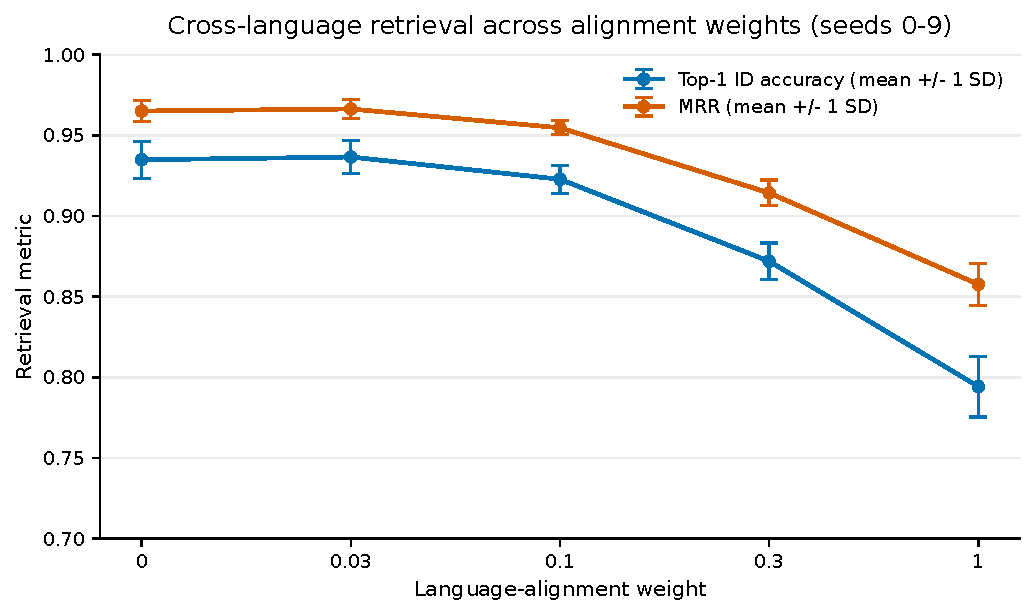
\includegraphics[width=0.84\linewidth]{bilingual_alignment_retrieval_sweep.pdf}
\caption{Cross-language proposition retrieval across language-alignment weights. Points show means across seeds 0--9, with error bars indicating $\pm$1 SD. Top-1 measures nearest-neighbour same-ID retrieval in the opposite language; MRR measures the rank of the correct match. Retrieval is already strong at $\lambda$ = 0.00 and is numerically slightly higher at $\lambda$ = 0.03, but the paired differences are small relative to seed variation. Performance declines under larger weights.}
\end{figure}

\begin{figure}[htbp]
\centering
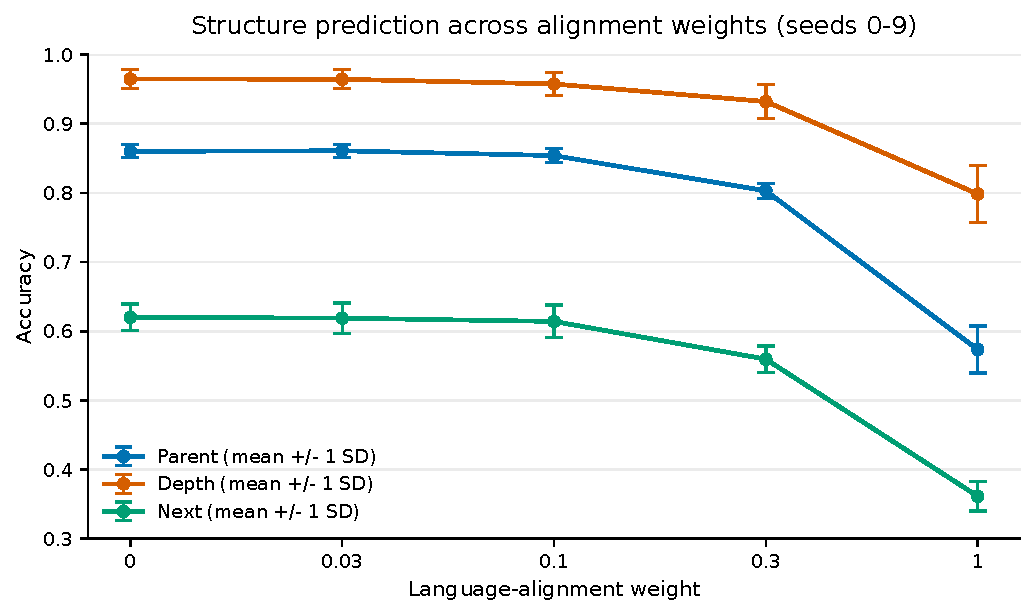
\includegraphics[width=0.94\linewidth]{bilingual_structure_accuracy_sweep.pdf}
\caption{Formal-position prediction accuracy across language-alignment weights. Points show means across seeds 0--9, with error bars indicating $\pm$1 sample SD. Depth has the highest raw accuracy, while successor has the largest observed class space; the three tasks are not directly comparable measures of difficulty. The no- and light-alignment settings are similar, and all three heads deteriorate as the weight becomes larger.}
\end{figure}

\begin{figure}[htbp]
\centering
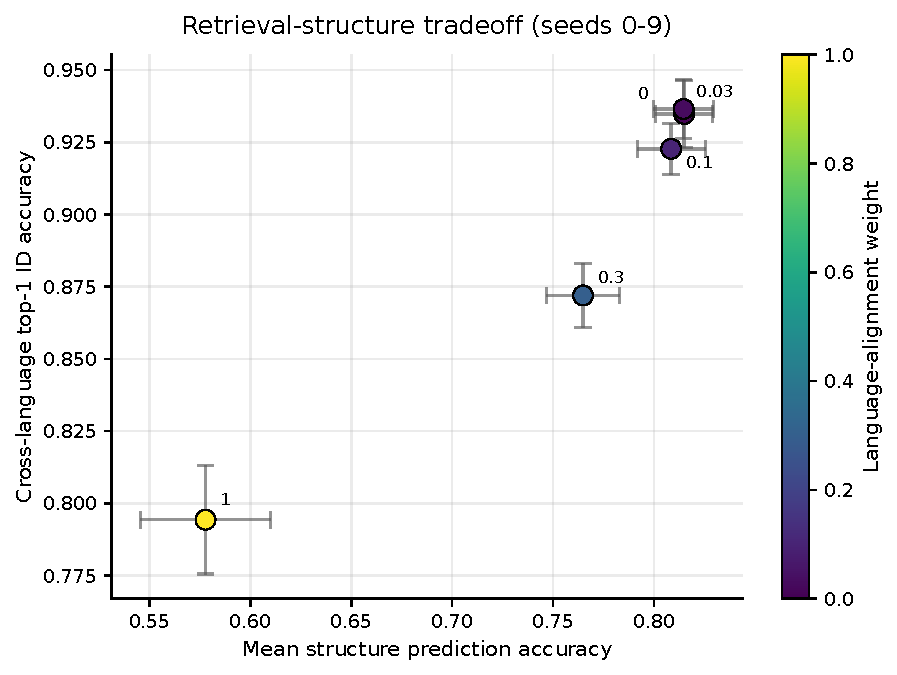
\includegraphics[width=0.88\linewidth]{bilingual_retrieval_structure_tradeoff.pdf}
\caption{Retrieval--structure trade-off across language-alignment weights. Each point represents the ten-seed mean for a $\lambda$ setting, with error bars showing $\pm$1 SD. The x-axis reports a descriptive mean of parent, depth, and successor accuracies; because the tasks differ in granularity, the composite is used only to display change across fixed conditions. The y-axis reports cross-language Top-1 proposition-ID retrieval. Low alignment occupies the upper-right region, whereas $\lambda$ = 1.00 gives the weakest combined performance.}
\end{figure}

\begin{figure}[htbp]
\centering
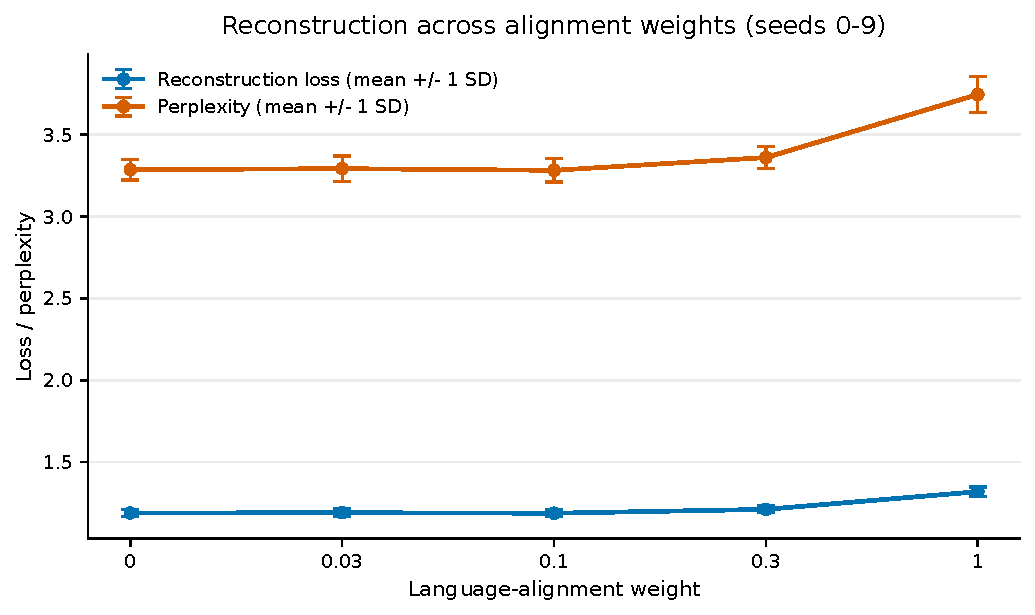
\includegraphics[width=0.88\linewidth]{bilingual_reconstruction_sweep.pdf}
\caption{Reconstruction diagnostics across language-alignment weights. Points show means across seeds 0--9, with error bars indicating $\pm$1 SD. Reconstruction remains broadly stable at low alignment, but worsens as $\lambda$ increases, especially at $\lambda$ = 1.00. Reconstruction is therefore a useful diagnostic but not sufficient for model selection.}
\end{figure}

\begin{figure}[htbp]
\centering
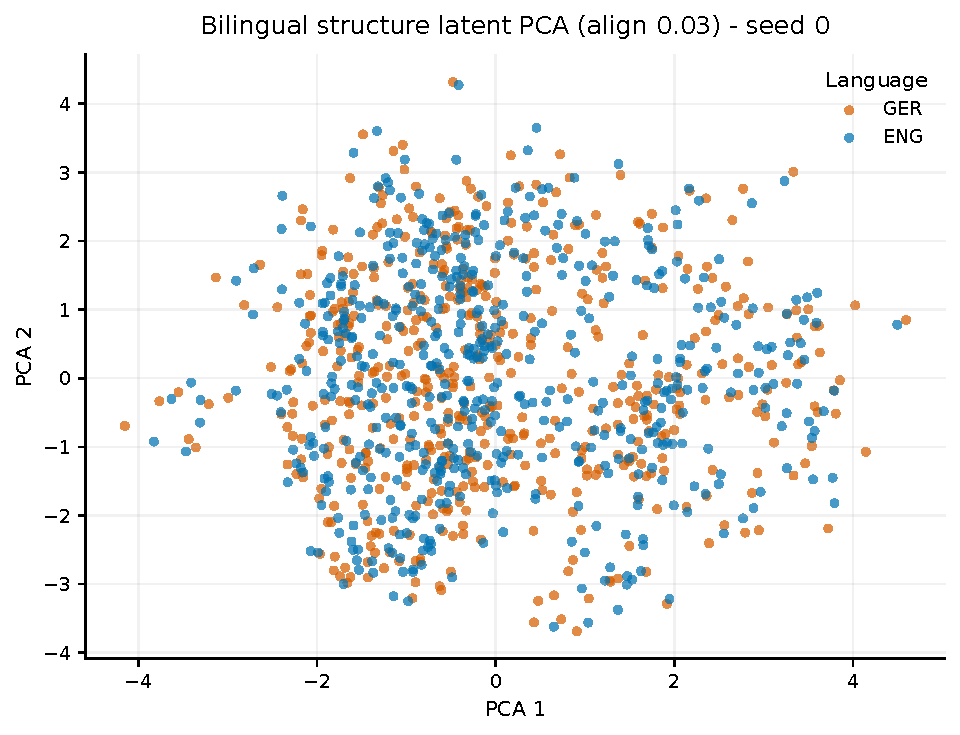
\includegraphics[width=0.94\linewidth]{bilingual_latent_pca_language_align003_seed000.pdf}
\caption{PCA projection of the bilingual 8-dimensional structure latent for the representative light-alignment condition $\lambda$ = 0.03, seed 0, coloured by language. German and English samples occupy the same broad regions rather than separating into language-specific clusters. This is a single-seed diagnostic, not evidence that $\lambda$ = 0.03 is decisively superior, and should be read alongside the ten-seed metrics.}
\end{figure}

\clearpage
\subsection{Exploratory Proposition-Family Demonstration}
The rule-based, text-blind selection procedure identified the immediate family under proposition 2.2: propositions 2.201, 2.202, 2.203, 2.21, and 2.22. Across ten monolingual seeds, the family's mean pairwise distance was 2.5324 $\pm$ 0.4181, compared with a mean of 5.2159 for depth- and branch-matched randomly assembled sets. None of the 5,000 matched sets per seed was at least as cohesive as the observed family. This matched-null result reflects the broader sibling-cohesion pattern rather than making family 2.2 uniquely compact: a post-selection comparison with the 55 eligible actual families placed it sixth highest in mean pairwise distance, and highest among the eight eligible five-child families. The case therefore combines formal-family cohesion relative to unrelated propositions with comparatively strong internal differentiation among actual families.

Proposition 2.22 was the most distant member in all ten seeds (Table 11 and Figure 7). Its mean distance to the other children was 3.2307 $\pm$ 0.5111; the corresponding values for 2.201, 2.202, 2.203, and 2.21 ranged from 2.1885 to 2.4810. This recurring differentiation is not necessarily a departure from the supplied scaffold. Proposition 2.22 is the only selected member with five direct children, whereas the other four are leaves, and the family contains both depth-three and depth-four propositions. Because depth and child count explicitly supervise the structure latent, the space may be distinguishing formal roles within a cohesive immediate family rather than identifying a textually anomalous proposition.

Once selected independently of its wording, the family nevertheless presents a useful object for close reading. Propositions 2.201--2.203 develop picturing through possible states of affairs and logical space; 2.21 turns to agreement or disagreement with reality and hence truth or falsity; and 2.22 states that what a picture represents is represented independently of its truth or falsity through the form of representation. Proposition 2.22 also opens a further five-proposition subfamily. Its recurrent latent differentiation therefore supplies a reproducible reason to ask whether it marks a change in expository or argumentative role. The model does not determine that interpretation, and because branching status is represented in the supervision, it is a plausible contributor to the observed separation \citep{wittgenstein1922tractatus}.

\begin{table*}[htbp]
\centering
\caption{Exploratory family 2.2 diagnostics from posterior structure means. Mean sibling distance is the mean $\pm$ sample SD across ten monolingual seeds. ``Farthest in seeds'' records how often the proposition had the largest mean distance to its siblings. Wider-neighbourhood Jaccard is the $\lambda$ = 0.00, $k$ = 10 cross-direction mean after excluding the known same-ID counterpart. The table reports representational diagnostics, not philosophical dependence.}
\resizebox{\textwidth}{!}{%
\begin{tabular}{lccccc}
\toprule
Proposition & Depth & Direct children & Mean sibling distance & Farthest in seeds & Wider-neighbourhood Jaccard \\
\midrule
2.201 & 4 & 0 & 2.1885$\pm$0.3521 & 0/10 & 0.5106 \\
2.202 & 4 & 0 & 2.4118$\pm$0.4472 & 0/10 & 0.5517 \\
2.203 & 4 & 0 & 2.3499$\pm$0.4632 & 0/10 & 0.5957 \\
2.21  & 3 & 0 & 2.4810$\pm$0.4979 & 0/10 & 0.6329 \\
2.22  & 3 & 5 & 3.2307$\pm$0.5111 & 10/10 & 0.5597 \\
\botrule
\end{tabular}%
}
\end{table*}

\begin{figure}[htbp]
\centering
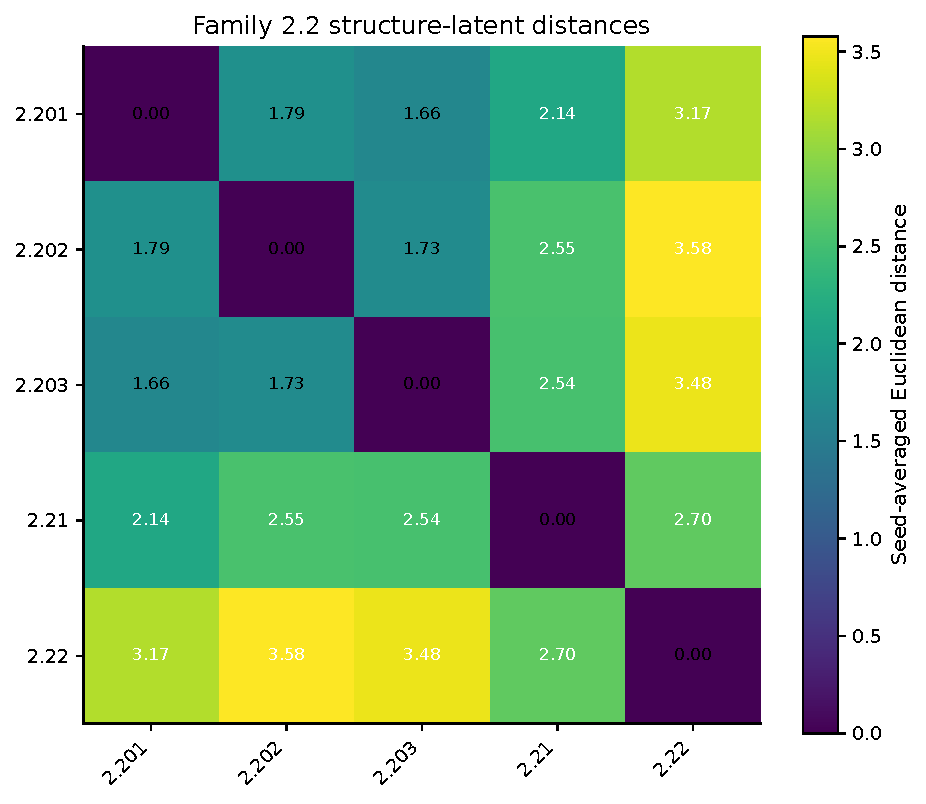
\includegraphics[width=0.96\linewidth]{family_case_distance_matrix.pdf}
\caption{Seed-averaged Euclidean distances between posterior structure means for the five immediate children of proposition 2.2. Proposition 2.22 is the most distant family member in all ten monolingual seeds. The distances describe the trained representation and should not be interpreted directly as philosophical dependence.}
\end{figure}

\section{Discussion}
The experiments support a methodological rather than an automated philosophical answer. In the monolingual setting, proposition wording contains retained-corpus signal about numbering-derived formal position and local family organisation. In the bilingual setting, German and English counterparts show strong correspondence in the shared structure space even without a direct same-ID alignment term. Because the numbering supplies the labels and the encoder receives proposition text, these findings do not amount to discovering the hierarchy from unlabeled material. They instead make the relation between textual realisation, formal position, and bilingual correspondence inspectable within a common representational framework.

The formal-position diagnostics probe different dimensions of organisation rather than directly comparable levels of difficulty. Depth is a coarse global label with six observed classes; parent prediction assigns propositions to 169 uneven immediate-parent classes; and successor prediction uses 526 nearly proposition-specific targets. Family organisation is assessed separately through sibling geometry rather than a classification head. The successor result is therefore informative even though its Top-1 accuracy is lower: the correct target appears within the top ten predictions in 0.8160 of cases. Child count supplies a further, but secondary, indication of branching information. Together, these diagnostics show that several dimensions of formal position are recoverable from wording within the fitted corpus, without establishing that hierarchy is philosophically prior to sequence.

Relational geometry adds evidence that is not reducible to label prediction. Sibling propositions are closer than unrelated propositions in every monolingual seed, with a mean unrelated-minus-sibling contrast of 3.4919. This indicates that local numbered families correspond to recurrent organisation in the learned space. Parent-child pairs are not uniformly close, however, so the geometry is not a Euclidean reconstruction of the decimal tree. It is better understood as a space of text-conditioned formal roles that can support family comparison, not as a direct measure of philosophical dependence.

The bilingual results show strong correspondence without identifying a single causal source. At $\lambda$ = 0.00, Top-1 retrieval is 0.9348 and MRR is 0.9650, substantially above both random ranking and the exact-input character n-gram reference. Direct same-ID attraction is therefore unnecessary within the shared architecture. The languages nevertheless share parameters, target spaces, mixed-corpus training, and surface cues, so the result cannot be attributed to hierarchy supervision alone. Importantly, the correspondence extends beyond recovery of the known counterpart: after that counterpart is excluded, the ten-neighbour wider-context Jaccard is 0.6240 $\pm$ 0.0086, compared with an expected value of approximately 0.0103 for independent random sets. The model thus supports comparison of surrounding proposition contexts across German and English, without establishing semantic equivalence.

The alignment sweep does not show a simple monotonic trade-off in which increasing $\lambda$ produces progressively stronger invariance at the expense of formal discrimination. The $\lambda$ = 0.00 and 0.03 conditions form a practically similar low-pressure regime: the light pairwise term slightly tightens matched posterior means while leaving retrieval and formal-position prediction largely unchanged. At higher weights, bilingual retrieval and formal-position discrimination deteriorate together, while same-ID distance also increases. This constitutes a high-weight failure regime, although the retained artefacts do not establish its mechanism.

The model does not provide an automated interpretation of the \emph{Tractatus}. Its scholarly value lies in converting the work's numbered organisation into a corpus-level object of comparison. Formal siblings, parent--child relations, sequential neighbours, and bilingual counterparts can be examined within a common represen\-tational framework, allowing researchers to identify cases that conform to or depart from expectations generated by the numbering scaffold. Those cases require philosophical and textual interpretation by scholars, but the model offers a reproducible way to locate and compare them. The present evidence is strongest for family comparison. Candidate departures and bilingual neighbourhoods should be treated as prompts for further inquiry, while hierarchy--sequence comparison currently remains aggregate because proposition-level parent and successor ranks were not retained.

The family 2.2 analysis demonstrates this workflow rather than supplying a philosophical conclusion. Selected through latent and formal diagnostics before its wording was examined, the family is cohesive relative to depth- and branch-matched random sets but comparatively dispersed among actual five-child families, while proposition 2.22 is its most distant member in all ten seeds. Yet 2.22 is also the family's only branching member and differs in depth from three of its siblings; both depth and child count are represented in the supervision. The result therefore identifies a stable case of formal-role differentiation for close reading, not a philosophical anomaly established by the model.

The transferable principle is that stable formal relations attached to substantial textual units can be used as weak supervision for text-conditioned comparison. Testing this principle beyond the \emph{Tractatus} would require reliable structural labels and controls for edition, translation, and surface overlap; cross-corpus transfer remains a future hypothesis rather than a result of this study.

\subsection{Limitations and Future Work}
The principal limitation is that the findings are retained-corpus diagnostics. No held-out propositions or families are used for the main claims, and the study examines one German and one English text. The labels are deterministic functions of proposition identifiers and corpus order, so the model learns a representation shaped by a supplied scaffold rather than discovering the numbered organisation or establishing its philosophical correctness. Stronger claims about generalisation require held-out family tests, additional editions or translations, and evaluation on other explicitly structured corpora.

The causal source of bilingual correspondence and the mechanism of high-weight deterioration both remain unresolved. At $\lambda$ = 0.00, vocabulary and model parameters, formal target spaces, mixed-corpus training, and the reconstruction objective remain shared, while exact-input lexical correspondence is non-trivial; the nearly proposition-specific successor objective may also provide a strong common signal. At positive $\lambda$, same-ID pairs contribute to the alignment loss only when both language versions occur in the same shuffled minibatch, and the necessary pair-coverage and optimisation trajectories were not retained. Future runs should therefore combine formal-head and shared-component ablations with paired or full-pair alignment implementations while retaining pair-coverage, latent-scale, and posterior-variance diagnostics.

The proposition-level demonstration is exploratory and uses the same fitted representations as the principal analyses. Family 2.2 differs internally in depth and child count, while its matched null uses randomly assembled propositions rather than actual families matched on every formal target; the post-selection actual-family comparison is not independent validation. Wider bilingual neighbourhoods are stable in aggregate, but individual lists vary with seed, neighbourhood size, and alignment condition; proposition-level parent and successor logits were not retained. Additional technical limitations include 96-token inputs, which truncate 121 of 1052 language-specific samples without isolating a causal truncation effect; post hoc child-count diagnostics for a strongly zero-skewed target; representative single-seed PCA projections; and an architecture that encourages but does not guarantee complete separation of the text and structure latents.

Future work should proceed in priority order. Causal attribution requires formal-position and shared-component ablations followed by controlled alignment implementations. Generalisation requires held-out proposition families, further translations and editions, and eventually external structured corpora. Stronger scholarly analysis requires prediction ranks for individual propositions, family matching on all supplied targets, and pre-specified comparisons of stable and divergent bilingual neighbourhoods. Graph-based structural baselines and more detailed length controls are useful extensions, but they do not replace these more immediate tests.

\section{Conclusion}
This study shows that proposition wording can be mapped into a text-conditioned structure space shaped by the numbered organisation of the \emph{Tractatus}. Parent, depth, successor, and child-count objectives shape the eight-dimensional structure latent, while sibling geometry provides relational evidence about local family organisation. These diagnostics recover distinct aspects of formal position within the retained corpus and should not be treated as a single scale of textual difficulty.

The bilingual experiment shows strong German--English correspondence within the shared architecture even when the explicit same-ID alignment loss is removed. Direct pairwise attraction is therefore unnecessary in this setting, although shared parameters, common target spaces, mixed training, and surface cues prevent attribution to hierarchy supervision alone. No or light alignment leaves formal-position discrimination largely intact, whereas heavy weighting damages correspondence and formal organisation together.

The scholarly contribution is methodological but interpretively enabling. The rule-based, text-blind family 2.2 analysis and wider bilingual-neighbourhood diagnostics show how the learned representation can locate cohesive, differentiated, and cross-language comparison cases within the \emph{Tractatus}. These diagnostics do not settle their philosophical or translational significance. They provide a reproducible route to case selection and comparison, while close reading remains responsible for interpretation.

\section*{Data and code availability}
Project code and derived experimental artefacts are available at:
\begin{flushleft}
\texttt{https://github.com/mark-alfred-griffiths/}\allowbreak
\texttt{Tractatus\_Logico\_Philosophicus\_Bilingual\_Study}
\end{flushleft}

\bibliographystyle{abbrvnat}
{\tolerance=2000 \hbadness=2000
\bibliography{references}
\par}

\end{document}
